\documentclass{article}
\usepackage{hyperref}
\usepackage{xcolor}
\usepackage{listings}	
\usepackage{amsmath,amssymb}
\usepackage{subcaption}
\usepackage{graphicx}
\usepackage{wrapfig}
\usepackage{geometry}
 \geometry{
 a4paper,
 total={170mm,257mm},
 left=10mm,
 right=10mm,
 top=10mm,
 }

\usepackage{tikz,ifthen}
\usetikzlibrary{shadings}
\usetikzlibrary{calligraphy}
\usetikzlibrary{intersections}
\usetikzlibrary{calc}
\usetikzlibrary{spy}
\usetikzlibrary{shadows,shapes.symbols}
\usetikzlibrary{intersections,perspective,decorations.pathreplacing,math}

\tikzset{spy using mag glass/.style={
  spy scope={
    every spy on node/.style={
      circle,
      fill, fill opacity=0.1, text opacity=1},
      every spy in node/.style={
        magnifying glass, circular drop shadow,
        fill=white, draw, ultra thick, cap=round},
      #1
    }
  }
}

\title{Supplementary material: Mandelbrot set}
\author{\href{https://github.com/cal-rmedina}{cal-rmedina}}
\date{}
\begin{document}
\maketitle

The following document describes the code implementation and the most important
funtions implemented in CUDA to generate the Mandelbrot set.

\section*{Output image}

 The output image size (\texttt{px}) is defined in the \verb|main| function,
the image size will be \verb|width|$\times$\verb|height| \texttt{px} (Fig.
\ref{fig:mandel1}), while the image dimensions can be chosen arbitrarily, it
must not exceed the available \textbf{GPU memory} (global memory). To ensure
this constraint, a function is included within the \verb|main| function
(\verb|limits(width,height);|). If the output dimensions exceed the available
memory, the code will terminate without completing the image computation. The
screen will display suitable parameters for the available GPU. However, it is
worth noting that modern GPUs generally provide sufficient memory to compute
big images in size ($>$ 2GB). The memory for the vector with size
\verb|size_vec = width*height*sizeof(int)|, used to compute each pixel color is
explicitly allocated on the GPU using \texttt{cudaMalloc}. 
A modification on the way to allocate memory should be made in order to compute
bigger images ($>$ GPU memory), having memory accessible by both; the CPU and
the GPU with \texttt{cudaMallocManaged} but that implementation is \textbf{out of the
scope of this simple code}.

\begin{figure}[h!]
  \centering
  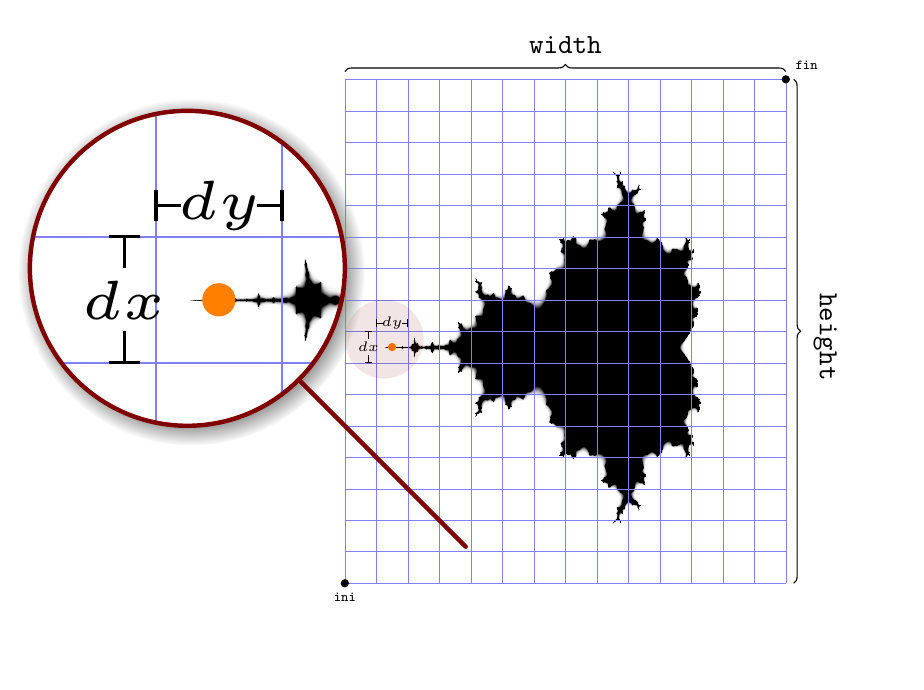
\begin{tikzpicture}[spy using mag glass={magnification=4.0, size=4cm}, 
    every spy in node/.style={magnifying glass, circular drop shadow,
    fill=white, draw, ultra thick, cap=round}]

    % Mandelbrot set
    \shade[shading=Mandelbrot set] (0.5,-1) rectangle (7,7);

    % Grid for pixels
    \draw[step=0.4, blue!50!white, very thin] (0.0,0.0) grid (5.6,6.41);

    % Braces: width & height
    \draw [decorate,decoration={brace}] (0,6.5) -- (5.6,6.5);
    \draw [decorate,decoration={brace, mirror}] (5.7,0) -- (5.7,6.4);

    % Labels: braces width & height
    \node[align=center, above] at (2.8,6.6) {\verb|width|};
    \node[align=center, left, rotate=-90 ] at (6.1,2.45) {\verb|height|};

    % Points: initial & final points in complex plane
    \fill[black] (0,0) circle (1.5pt);
    \fill[black] (5.6,6.4) circle (1.5pt);

    % Labels: points initial & final points in complex plane
    \node[align=center, below] at (0.0,0.0) {\tiny\verb|ini|};
    \node[align=center, above right] at (5.6,6.4) {\tiny\verb|fin|};

    \spy[red!50!black] on (0.5,3.1) in node at (-2.0,4.0);

    % Size of a pixel: dx & dy
    \draw[-, line width=0.3pt] (0.3,2.8) -- (0.3,2.9);
    \draw[-, line width=0.3pt] (0.3,3.1) -- (0.3,3.2);
    \draw[-, line width=0.3pt] (0.25,2.8) -- (0.35,2.8);
    \draw[-, line width=0.3pt] (0.25,3.2) -- (0.35,3.2);

    \draw[-, line width=0.3pt] (0.4,3.3) -- (0.48,3.3);
    \draw[-, line width=0.3pt] (0.72,3.3) -- (0.8,3.3);
    \draw[-, line width=0.3pt] (0.4,3.25) -- (0.4,3.35);
    \draw[-, line width=0.3pt] (0.8,3.25) -- (0.8,3.35);

    \node[font=\fontsize{0.4pt}{0}\selectfont] at (0.3,3.0) {$dx$};
    \node[font=\fontsize{0.4pt}{0}\selectfont] at (0.6,3.3) {$dy$};

    % Point: pixel
    \fill[orange] (0.6,3.0) circle (1.5pt);

  \end{tikzpicture}
  \caption{\textcolor{blue}{Squares} represent \texttt{pixels} and the \textcolor{orange}{point} is the complex number taken to compute the Mandelbrot set.}
  \label{fig:mandel1}
\end{figure}

The output image will have the dimension of \verb|width| $\times$ \verb|height|
pixels, the size of each \texttt{pixel} will be determined by the delimiting
points of the rectangular area in the complex plane given by $dx=\left( x_{fin}
- x_{ini} \right) / \verb|width|$ and $dy=\left( y_{fin} - y_{ini} \right)/
\verb|height|$. It can be seen (Fig. \ref{fig:mandel1}) that rectangular
pixels are possible ($dx\neq dy$), but the value computed will be the center
of the rectangular/square area.

\section*{2D Block arrange}
The Mandelbrot set is situated in the
\href{https://en.wikipedia.org/wiki/Complex_plane}{complex plane}, spanning
from the point \verb|ini| to \verb|fin|, where the coordinates of \verb|ini|
and \verb|fin| represent the lower and upper bounds of the rectangular region
that contains the set respectively, to cover the entire image, a kernel with 2D
\verb|blocks| is launched. Each block contains a fixed number of threads:
\verb|thrX=16| and \verb|thrY=16|, totaling 256 threads per block. The
condition that the \verb|width| and \verb|height| must be multiples of
\verb|thrX| and \verb|thrY| respectively ensures uniform distribution of
threads across the entire image without leaving any gaps.  With the thread size
fixed (\verb|thrX|,\verb|thrY|$=2^4$) it has been decided to use the  
\href{https://en.wikipedia.org/wiki/Bitwise_operations_in_C}{bitwise left
shift operation} to set the \verb|width| and \verb|height| values, as an
example for \verb|width=1<<10| (\verb|width=|$2^{10}$) and \verb|height=1<<10|
(\verb|height|=$2^{10}$).  For more detail of the block and
thread division check Fig. \ref{fig:mandel}.

\begin{figure}[h!]
  \centering
  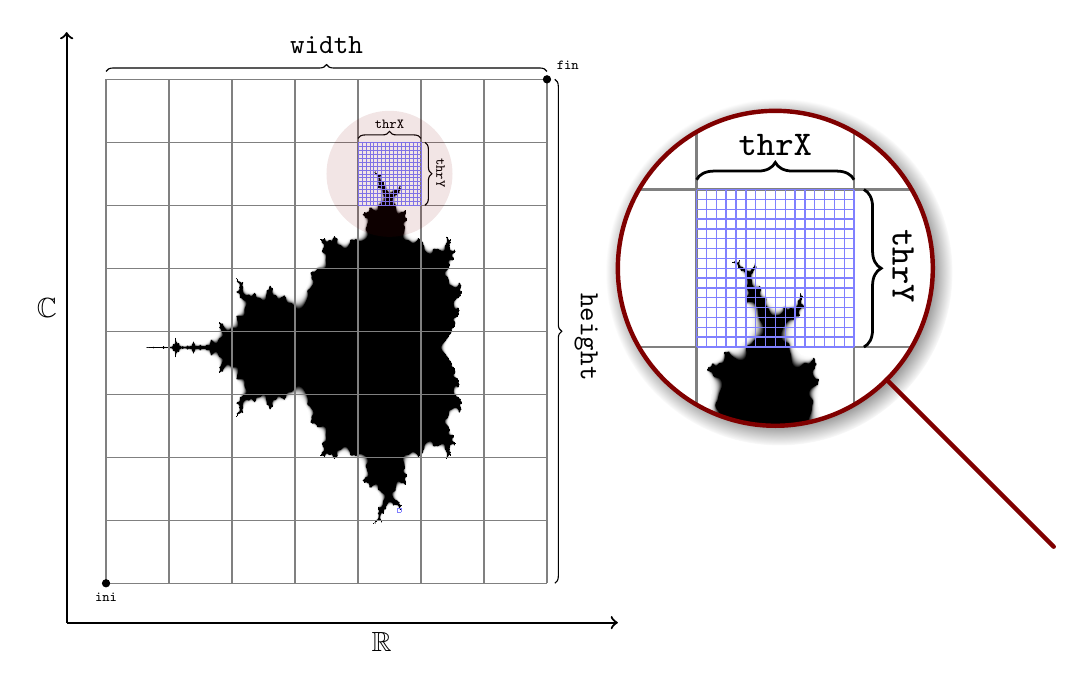
\begin{tikzpicture}[spy using mag glass={magnification=2.5, size=4cm}, 
    every spy in node/.style={magnifying glass, circular drop shadow,
    fill=white, draw, ultra thick, cap=round}]

    % Mandelbrot set
    \shade[shading=Mandelbrot set] (0.5,-1) rectangle (7,7);

    % Axis: complex plane
    \draw[thick,->] (-0.5,-0.5) -- (6.5,-0.5);
    \draw[thick,->] (-0.5,-0.5) -- (-0.5,7.0);

    % Labels: axis complex plane
    \node[align=center, below] at (3.5,-0.5) {$\mathbb{R}$};
    \node[align=center, left] at  (-0.5,3.5) {$\mathbb{C}$};

    % Grid covering Mandelbrot set
    \draw[step=0.8,gray] (0,0) grid (5.6,6.4);

    % Grid for the zoom spy
    \draw[step=0.05, blue!50!white, very thin] (3.2,4.8) grid (4.0,5.6);

    % Grid for pixel zoom spy
    \draw[step=0.05, blue!50!white, very thin] (3.7,0.9) grid (3.75,0.95);

    % Braces: width & height
    \draw [decorate,decoration={brace}] (0,6.5) -- (5.6,6.5);
    \draw [decorate,decoration={brace, mirror}] (5.7,0) -- (5.7,6.4);

    % Labels: braces width & height
    \node[align=center, above] at (2.8,6.6) {\verb|width|};
    \node[align=center, left, rotate=-90 ] at (6.1,2.45) {\verb|height|};

    % Braces: thrX & thrY
    \draw [decorate,decoration={brace}] (3.2,5.65) -- (4.0,5.65);
    \draw [decorate,decoration={brace,mirror}] (4.05,4.8) -- (4.05,5.6);

    % Labels: braces thrX & thrY
    \node[align=center, above] at (3.6,5.65) {\tiny\verb|thrX|};
    \node[align=center, left, rotate=-90] at (4.25,4.9) {\tiny\verb|thrY|};

    % Points: initial & final points in complex plane
    \fill[black] (0,0) circle (1.5pt);
    \fill[black] (5.6,6.4) circle (1.5pt);

    % Labels: points initial & final points in complex plane
    \node[align=center, below] at (0.0,0.0) {\tiny\verb|ini|};
    \node[align=center, above right] at (5.6,6.4) {\tiny\verb|fin|};

    \spy[red!50!black] on (3.6,5.2) in node at (8.5,4.0);

  \end{tikzpicture}
  \caption{Within the grid, individual squares correspond to distinct objects,
  a gray square represents a \texttt{block}, while a blue square a
  \texttt{pixel}, rectangular arranges are also possible.}
  \label{fig:mandel}
\end{figure}

Increasing the number of pixels will lead to a more detailed output image but
it also increases the size, a comparison for the same region increasing the
number of pixels can be seen in Fig. \ref{fig:pixel}, if a more detailed output
image is desired or plotting a different section is needed, the points
\verb|ini| and \verb|fin| can be changed to reduce/increase the area computed. 

\begin{figure}[h!]
  \centering
  \begin{subfigure}[t]{0.3\linewidth}
    \includegraphics[width=1.0\textwidth]{mb_512.png}
    \caption{$512\times 512$ \texttt{px}}
  \end{subfigure}
  \begin{subfigure}[t]{0.3\linewidth}
    \includegraphics[width=1.0\textwidth]{mb_1024.png}
    \caption{$2048\times 2048$ \texttt{px}}
  \end{subfigure}
  \begin{subfigure}[t]{0.3\linewidth}
    \includegraphics[width=1.0\textwidth]{mb_4096.png}
    \caption{$4096\times 4096$ \texttt{px}}
  \end{subfigure}
  \caption{Images with square region increasing the number of pixels.}
  \label{fig:pixel}
\end{figure}

\end{document}
